\subsection{Diseno}
Para realizar una buena seleccion en el conjunto de datos de los campos que son relevantes o la combinacion de estos, es imprescindible unos 
conocimientos solidos sobre la materia a tratar. Por ello, es fundamental dedicarle el tiempo necesario para enter la
importancia del concepto, que beneficios nos puede aportar o que situaciones nos perjudican.
Los puntos que deben quedar claro en la fase de diseno son:\\

 \textbf{Objetivo}. Conceptualmente, que problema queremos solventar o clarificar. Es muy importante que tengamos un objetivo claro,
    incluso si no se cuentan con conocimientos previos de la materia, tener un objetivo bien definido nos ayuda a encontrar la solucion o 
    describirla con mas claridad al experto para que este nos describa como solventar el problema.\\

 \textbf{Puntos importantes. Situaciones destacables}. Como mencionamos anteriormente, nuestro objetivo no es mostrar todos los valores, sino
    que se trata de proporcionarle la informacion importante al usuario para poder descubrir las situaciones significativas, los que tienen influencia en
    nosotros, ya sea positivo o negativo. A nivel mas tecnico, serian los limites o que valores de que datos son los que nos proporcinan una informacion
    de una situacion excepcional, o los valores que estamos intentando identificar mas facilmente.\\

 \textbf{Data workflow}. Diseno del flujo de informacion, que quede claro como se llega de un punto a otros, por ejemplo de una representacion
    simple a mas detallada o compleja. Si el usuario entiende los conceptos basicos, le sera mas facil de entender el concepto mas desarrollado.

\subsubsection{How to solve it} 
Una vez marcada una meta, deberemos estipular cuales son los campos necesarios del conjunto de datos que necesitamos para representar la informacion
disenada.Es decir, realizamos la seleccion de los campos que nos interesen. Es momento de realizar un analisis de los datos proporcionados y ver en 
la lista de los campos que nos ofrece la fuente, si serian suficientes para alcanzar el objetivo marcado, si no directamente con sus valores, con la combinacion de ellos.
A continuacion estipulamos los valores destacables que les proporcionen mas informacion al usuario como las situaciones excepcionales, o lo que estamos buscando.
\subsubsection{How we solve it. Aire Guru} 
Nuestro objetivo principal es crear el concienciamiento de la importancia de la polucion del aire en nuestra salud. Para ello investigamos diferentes conceptos:
\begin{itemize}
    \item Que enfermedades se ven afectadas por la polucion del aire
    \item Que contaminantes son las que crean o influyen en enfermedades
    \item Cuales son las fuentes de cada contaminante
    \item Cual es la medida representativa del nivel de polucion del aire.
    \item Como se calcula y que parametros necesitamos para su calculo
    \item Cuales son los niveles nocivos en general y para cada contaminante
\end{itemize}
La medida que mejor representa el nivel de polucion en el aire, en este caso es el AQI. Investigamos sobre ello en fuentes oficiales, para la ciudad de Malaga se aplica la 
legislacion europea, por lo que nos centramos en esta normativa.
Buscamos las relaciones que tienen los contaminantes con distintas enfermedades, para ello recurrimos a estudios clinicos. Para cada una de las enfermedades, nos informamos
sobre sus sintomas y como se pueden ver agravados por cada contaminante.
Para cada contaminante, buscamos las fuentes de polucion y vemos si se aplican a la ciudad de Malaga y como.
Con toda esta informacion definimos que los contaminantes que afectan a la calidad del aire son el CO, NO2, O3 y PM (Particulated Material), diferentes medidas de particulas
afectan de distinto modo a distintas enfermedades.\\

Como el objetivo principal es la concienciacion, aportaremos todos estos datos de una manera organizada en el glosario de Aire Guru.\\

Una vez seleccionados estos contaminantes, verificamos si contamos con estos datos en nuestro conjunto de datos. Como mencionamos anteriormente algunas muestras
muestran medidas de estaciones fijas y/o moviles y estas pueden ser cuantitativas o cualitativas y otras no cuentan con las medidas. Deberemos seleccionar la que
nos aporte la mayor informacion o la que sea mas precisa, en este caso prevalecera la medida cuantitativa a la cualitativa y en el caso de que solo haya cualitativa
se deciden los siguientes valores Bueno:50, Aceptable:150,Pobre:300, Malo:400, Insalubre:500 y se le indicara al usuario cuando el valor es cualitativo.\\


En este punto que sabemos como afecta la polucion del aire en nuestra salud, vamos a dejar claro en nuestras representaciones cuales son los valores indeseables,
para ello utilizamos los colores de alerta, amarillo, naranja y rojo, estos colores se eligen en la paleta de los colores proporcionados por el EAQI.
Se utiliza la altura en las graficas, ya que es una representacion intuitiva para el ser humano. Ademas el icono que representa una polucion insalubre, es 
totalmente distinto y busca la sensacion de alarma, para evocar en el usuario una sensacion de peligro.\\
\newpage
\begin{figure}[ht]
    \centering
   \subfigure[BarChart Aire Guru]
    {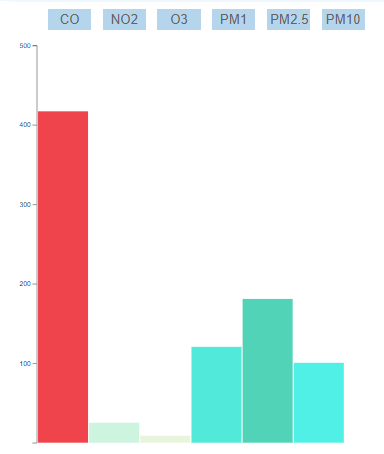
\includegraphics[width=5cm  ]{barchart}}
    \hfill
    \subfigure [Categoria medio ambiente]
       { 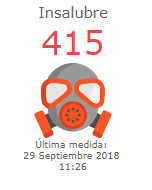
\includegraphics[width=4cm]{unhealthyIcon}}
  
  \caption{Alert situation}
    \end{figure}

Respecto al workflow, vamos guiando al usuario desde la seleccion de un punto en la ciudad de Malaga, ya sea por iniciativa propia 
o automatica a los detalles de este punto a tiempo real y continuamos por mostrarle la evolucion de la polucion en ese punto.
La logica de este desarrollo es que se prevee que el usuario estara interesado en la polucion que le rodea a tiempo real y si 
quiere saber el desglose de los contaminantes en el punto donde se encuentra, puede continuar indagando. El mapa, ademas de mostrar
el punto donde se encuentra el usuario sirve de verificacion, da mas realismo y confianza al usuario.

\elsparagraph{Evaluation}  
\begin{itemize}
    \done La definicion del objetivo es clara y se ha realizado una investigacion que nos proporciona la informacion necesaria
    para saber si podemos utilizar el conjunto de datos o no.
    \done Los niveles preocupantes se han definido como pobre, malo e insalubre y son representados en la herramienta Aire Guru
    claramente para que el usario sea capaz de localizarlos rapidamente.
    \done El workflow es satisfactorio, ya que el usuario sabe de un simple vistazo donde esta y el nivel de polucion en ese punto 
    y puede escrudinar la informacion facilmente si lo desea.
    
\end{itemize}
 

\newpage